\documentclass[12pt,letterpaper]{article}

\usepackage[titletoc]{appendix}
\usepackage[compatibility=false]{caption}

\usepackage{fullpage, listings, footnote, graphicx, multicol, enumitem, latexsym, placeins, csvsimple}
\usepackage{algorithm,algpseudocode}

\usepackage[backend=biber,style=numeric]{biblatex}

\usepackage{hyperref}
\usepackage{cleveref}

\usepackage{amsmath}

\DeclareLanguageMapping{american}{american-apa}
\addbibresource{Lab2.bib}

\setdescription{leftmargin=\parindent,labelindent=\parindent}
\pdfpxdimen=\dimexpr 1 in/72\relax
\lstdefinestyle{appendixJava}{%
  belowcaptionskip=1\baselineskip,
  breaklines=true,
  xleftmargin=\parindent,
  xrightmargin=\parindent,
  language=Java,
  showstringspaces=false,
  basicstyle=\small,
  numberstyle=\tiny,
  keywordstyle=\bfseries,
  commentstyle=\itshape,
  numbers = left,
  tabsize=4,
}
\lstdefinestyle{log}{%
  belowcaptionskip=1\baselineskip,
  breaklines=true,
  frame=tb,
  xleftmargin=\parindent,
  xrightmargin=\parindent,
  showstringspaces=false,
  basicstyle=\footnotesize\ttfamily,
  tabsize=4,
}
\author{Hawk Weisman\\CMPSC440: Operating Systems}
\title{Lab 5: Using Simulation to Evaluate Scheduling Algorithms}
\date{Monday, March 10th, 2014}
\begin{document}
	\maketitle
	\tableofcontents
  	\section{Introduction}

  		Scheduling algorithm selection is an extremely important decision in operating system design. Choosing a process scheduler can have significant influence on system performance metrics such as wait time, response time, and turnaround time. However, the workloads which these algorithms must schedule vary sigificantly, they are difficult to study analytically. Simulation, therefore, is a useful tool for investigating the performance of various scheduling algorithms.

  	\section{Methods}

  		\subsection{Simulation \& Metrics}
	  		A CPU simulator implemented by Jim Weller was used to assess various scheduling algorithms. The simulator is available at \url{http://jimweller.com/jim-weller/jim/java_proc_sched/}.

	  		\begin{figure}[H]
				\centerline{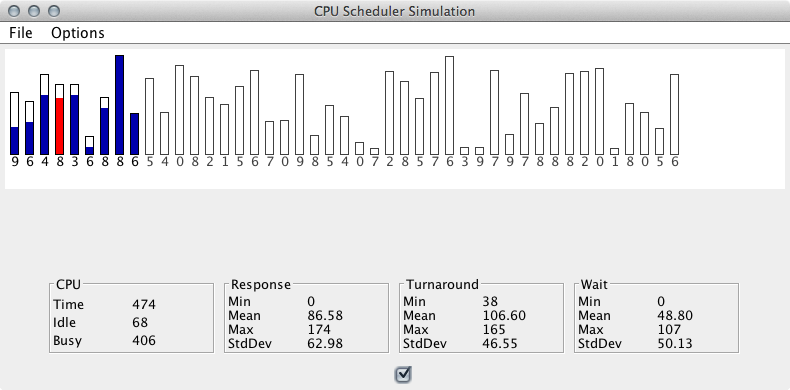
\includegraphics[width=0.80\textwidth]{figures/sim.png}}
				\caption{A screenshot of the CPU simulator implemented by Jim Weller.}
				\label{fig:screenshot}
			\end{figure}

			Seven scheduling algorithms were tested: first come, first serve; preemptive and non-preemptive priority; prioritized and non-prioritized round-robin; and preemptive and non-preemptive shortest job first. 
			\subsubsection{Summary of Scheduling Algorithm}
			\begin{description}[leftmargin=4cm, style=multiline]
					\item[First come, first served]{Also known as \textit{first in, first out}. Probably the simplest scheduling algorithm, this algorithm simply executes jobs in order of their arrival in the ready queue.}
					\item[Shortest job first]{This algorithm schedules jobs in order of length, executing the shortest jobs first.}
						\begin{description}[style=nextline, font=\normalfont\itshape]
							\item[non-preemptive]{In this variant, once a job has begun executing, it will continue executing until it has finished.}
							\item[preemptive]{Unlike the non-preemptive variant, if a job which is shorter than the current job arrives in the ready queue, this algorithm will stop executing the current job and begin executing the shorter job.}
						\end{description}
					\item[Priority]{This algorithm schedules jobs according to priority, executing the highest-priority jobs first.}
						\begin{description}[style=nextline, font=\normalfont\itshape]
							\item[non-preemptive]{In this variant, once a job has begun executing, it will continue executing until it has finished.}
							\item[preemptive]{Unlike the non-preemptive variant, if a job with a higher priority than current job arrives in the ready queue, this algorithm will preempt execution of the current job and begin executing the higher-priority job.}
						\end{description}
					\item[Round robin]{Round robin scheduling assigns each process a \textit{time quantum}, or amount of time over which it may execute, and allows each process in the ready queue to execute for the time quantum in order. If a job is not finished at the end of the time quantum, the scheduler interrupts it and allows the next job to execute. It will then be allowed to resume execution once the scheduler reaches its position in the queue again.}
						\begin{description}[style=nextline, font=\normalfont\itshape]
							\item[non-prioritized]{The non-prioritized round robin variant rotates between all jobs in the ready queue, regardless of priority.}
							\item[prioritized]{The prioritized round robin variant preferrentially rotates between all of the highest priority jobs. If there are no jobs of the highest priority in the ready queue, it will try to alternate between jobs of the next-highest priority level.} 
						\end{description}
				\end{description}

			The CPU simulator recorded the time when each simulated process arrived in the ready queue, when it began execution, and when it finished. This allows for the calculation of the following performance metrics:
				\begin{description}[leftmargin=4.5cm, style=sameline]
					\item[Response Time]{The amount of time between when a job is started and when the first response is produced.}
					\item[Wait Time]{The amount of time a job spends in the ready queue before it may begin execution.}
					\item[Turnaround Time]{The amount of time between when a job arrives in the ready queue and when it completes execution.}
				\end{description}

			Formally, we can define these metrics with the following equations:
				\begin{align*}
				  	T_{response} &= T_{response} - T_{submission}\\
					T_{turnaround} &= T_{completion} - T_{submission}\\
					T_{wait} &= T_{start} - T_{submission}
				\end{align*}
			All of these are measurements of performance, and lower values are better.

			Multiple data sets were used in this study: one provided by Jim Weller for download at \url{http://jimweller.com/jim-weller/jim/java_proc_sched/}, and five which were run from randomly-generated workloads produced using the random workload setting in the CPU simulator tool.

		\subsection{Data Analysis \& Visualization}
			Data collected from the simulation was analyzed using the IPython interactive computing environment \cite{ipython}, using the Pandas library \cite{ pandas} for statistical analysis. Visualizations were prepared using Matplotlib \cite{matplotlib}. A static copy of the IPython notebook used to analyze and visualize the data may be viewed at \url{http://nbviewer.ipython.org/gist/hawkw/9439505}.

			Box-and-whisker plots (\cref{fig:jim_whisker_response,fig:jim_whisker_wait,fig:jim_whisker_turn})) were produced to show the distribution of the data collected for each scheduling algorithm.

  	\section{Results \& Analysis}

  		\Cref{table:data-jim} summarizes the dataset downloaded from \url{http://jimweller.com/jim-weller/jim/java_proc_sched/}.

  		\begin{table}
  			\label{table:data-jim}
  			\caption{Data from \url{www.jimweller.com}}
	  		\begin{tabular}{l r r r r}
				\textbf{Shortest Job First} & mean & standard deviation & minimum & maximum\\
				\hline
Wait time &		23.4 &	33.1499622926 &	0 &	0 	\\
Response time &		23.4 &	33.1499622926 &	0 &	147 	\\
Turnaround time &	54.02 &	48.4555425106 &	3 &	246 	\\
				\\
				\textbf{Shortest Job First (preemptive)} \\
				\hline
Wait time &		18.24 &	38.6717261058 &	0 &	0 	\\
Response time &		13.68 &	31.2681563256 &	0 &	147 	\\
Turnaround time &	48.86 &	56.9677136631 &	3 &	286 	\\
				\\
				\textbf{First Come, First Serve} \\
				\hline
Wait time &		34.7 &	43.2301977789 &	0 &	0 	\\
Response time &		34.7 &	43.2301977789 &	0 &	156 	\\
Turnaround time &	65.32 &	49.252995848 &	3 &	196 	\\
				\\
				\textbf{Round-robin} \\
				\hline
Wait time &		39.96 &	48.3060907133 &	0 &	0 	\\
Response time &		7.64 &	11.329183554 &	0 &	46 	\\
Turnaround time &	70.58 &	65.1457105265 &	3 &	296 	\\
				\\
				\textbf{Round-robin (prioritized)} \\
				\hline
Wait time &		41.6 &	49.9159293212 &	0 &	0 	\\
Response time &		27.44 &	31.9137337208 &	0 &	108 	\\
Turnaround time &	72.22 &	60.8411998567 &	3 &	250 	\\
				\\
				\textbf{Priority} \\
				\hline
Wait time &		28.52 &	57.4387465044 &	0 &	0 	\\
Response time &		28.52 &	57.4387465044 &	0 &	363 	\\
Turnaround time &	59.14 &	65.0744220105 &	3 &	386 	\\
				\\
				\textbf{Priority (preemptive)} \\
				\hline
Wait time &		34.34 &	84.741161191 &	0 &	0 	\\
Response time &		18.2 &	55.246357346 &	0 &	363 	\\
Turnaround time &	64.96 &	95.8546733342 &	3 &	528 	\\

				\\
			\end{tabular}
		\end{table}

  	  	\begin{figure}[H]
			\centerline{\includegraphics[width=\textwidth]{figures/weller_whisker_response.pdf}}
			\caption{Box-and-whisker plot of response time (\url{www.jimweller.com} data).}
			\label{fig:jim_whisker_response}
		\end{figure}

		\begin{figure}[H]
			\centerline{\includegraphics[width=\textwidth]{figures/weller_whisker_wait.pdf}}
			\caption{Box-and-whisker plot of wait time (\url{www.jimweller.com} data).}
			\label{fig:jim_whisker_wait}
		\end{figure}

		\begin{figure}[H]
			\centerline{\includegraphics[width=\textwidth]{figures/weller_whisker_turnaround.pdf}}
			\caption{Box-and-whisker plot of turnaround time (\url{www.jimweller.com} data).}
			\label{fig:jim_whisker_turn}
		\end{figure}

  	\section{Discussion}

  		\subsection{Assessment of Scheduling Algorithms}


  		\subsection{Difficulties \& Opportunities for Further Study}
  			A major flaw in this study is that the metrics collected (response time, wait time, and turnaround time) are all measurements of \textit{performance}. While performance is a major concern in the implementation of schedulers, operating systems designers are also interested in other characteristics, such as \textit{fairness}, ensuring that equal CPU time is distributed to each process (or, in systems with priority, according to its priority and workload); \textit{throughput}, the total number of processes that complete execution over a given time interval, and \textit{utilization}, ensuring that the most efficient possible use is made of the CPU and other system resources. A more comprehensive study of scheduling algorithms might record information on these qualities as well.

  			Another issue is that of \textit{representativeness}. Since  simulation-based studies by definition do not involve data collected from real-world machines, it is important to ensure that the inputs to the simulation are representative of the actual conditions under which the algorithms under study must function. In the case of scheduling algorithms, this means that the characteristics of the workload, such as the burst time, or amount of CPU time each process requires to execute; the delay in the rate at which new processes enter the ready queue; and the distribution of priorities assigned to processes entering the ready queue, must all be made as close as possible to the characteristics of the workloads on real-world machines. Otherwise, the results of the simulation will not be very valuable for making decisions in the real world.

  			More representative simulation inputs might be prepared by conducting observations of the workload characteristics of a wide range of actual computers, analyzing those observations, and constructing a workload or set of workloads based on the patterns found in these observations. Those workloads could then be used as input to simulations with the understanding that they represent with some accuracy the conditions under which scheduling algorithms will actually operate.

	\begin{appendices}

		\section{Data}
			\label[appendix]{app:data}

			\addcontentsline{toc}{subsection}{Random Workload I}
			\begin{table}[H]
	 			\label{table:data-rand1}
	  			\caption{Data from the first random workload.}
		  		\begin{tabular}{l r r r r}
					\textbf{Shortest Job First} & mean & standard deviation & minimum & maximum\\
					\hline
					Wait time &		343.42 &	551.749112913 &	0 &	0 	\\
					Response time &		343.42 &	551.749112913 &	0 &	2067 	\\
					Turnaround time &	394.66 &	572.012328888 &	24 &	2162 	\\
					\\
					\textbf{Shortest Job First (preemptive)} \\
					\hline
					Wait time &		335.64 &	557.678680245 &	0 &	0 	\\
					Response time &		326.82 &	560.773347797 &	0 &	2067 	\\
					Turnaround time &	386.88 &	578.559785675 &	3 &	2162 	\\
					\\
					\textbf{First Come, First Serve} \\
					\hline
					Wait time &		583.64 &	272.881421867 &	0 &	0 	\\
					Response time &		583.64 &	272.881421867 &	0 &	993 	\\
					Turnaround time &	634.88 &	269.476428654 &	65 &	999 	\\
					\\
					\textbf{Round-robin} \\
					\hline
					Wait time &		860.24 &	517.426074333 &	1 &	1 	\\
					Response time &		82.94 &	71.8894734993 &	0 &	298 	\\
					Turnaround time &	911.48 &	541.01261501 &	11 &	1914 	\\
					\\
					\textbf{Round-robin (prioritized)} \\
					\hline
					Wait time &		830.4 &	670.613778564 &	45 &	45 	\\
					Response time &		287.26 &	112.772658034 &	0 &	466 	\\
					Turnaround time &	881.64 &	686.207658366 &	80 &	2137 	\\
					\\
					\textbf{Priority} \\
					\hline
					Wait time &		584.94 &	630.010203409 &	0 &	0 	\\
					Response time &		584.94 &	630.010203409 &	0 &	2365 	\\
					Turnaround time &	636.18 &	628.436876385 &	18 &	2405 	\\
					\\
					\textbf{Priority (preemptive)} \\
					\hline
					Wait time &		600.24 &	635.131909449 &	0 &	0 	\\
					Response time &		562.94 &	647.064831682 &	0 &	2365 	\\
					Turnaround time &	651.48 &	634.430145564 &	15 &	2405 	\\
					\\
				\end{tabular}
			\end{table}

			\addcontentsline{toc}{subsection}{Random Workload II}
			\begin{table}[H]
	 			\label{table:data-rand2}
	  			\caption{Data from the second random workload.}
		  		\begin{tabular}{l r r r r}
					\textbf{Shortest Job First} & mean & standard deviation & minimum & maximum\\
					\hline
Wait time &		426.02 &	661.628944046 &	0 &	0 	\\
Response time &		426.02 &	661.628944046 &	0 &	2399 	\\
Turnaround time &	482.78 &	681.05621765 &	8 &	2492 	\\
					\\
					\textbf{Shortest Job First (preemptive)} \\
					\hline
Wait time &		417.32 &	676.881716107 &	0 &	0 	\\
Response time &		400.6 &	672.674007228 &	0 &	2399 	\\
Turnaround time &	474.08 &	696.785787456 &	1 &	2492 	\\
					\\
					\textbf{First Come, First Serve} \\
					\hline
Wait time &		677.76 &	329.807068451 &	0 &	0 	\\
Response time &		677.76 &	329.807068451 &	0 &	1070 	\\
Turnaround time &	734.52 &	326.00596559 &	8 &	1155 	\\
					\\
					\textbf{Round-robin} \\
					\hline
Wait time &		1013.34 &	562.567564298 &	0 &	0 	\\
Response time &		96.08 &	79.6765561505 &	0 &	303 	\\
Turnaround time &	1070.1 &	588.339706292 &	8 &	1974 	\\
					\\
					\textbf{Round-robin (prioritized)} \\
					\hline
Wait time &		912.66 &	666.017885946 &	0 &	0 	\\
Response time &		386.0 &	181.003093896 &	0 &	914 	\\
Turnaround time &	969.42 &	680.328129361 &	8 &	2540 	\\
					\\
					\textbf{Priority} \\
					\hline
Wait time &		691.06 &	691.35957099 &	0 &	0 	\\
Response time &		691.06 &	691.35957099 &	0 &	2376 	\\
Turnaround time &	747.82 &	688.458733404 &	8 &	2457 	\\

					\\
					\textbf{Priority (preemptive)} \\
					\hline
Wait time &		698.86 &	689.455901708 &	0 &	0 	\\
Response time &		683.2 &	698.788379984 &	0 &	2376 	\\
Turnaround time &	755.62 &	686.830281511 &	8 &	2457 	\\
					\\
				\end{tabular}
			\end{table}

			\addcontentsline{toc}{subsection}{Random Workload III}
			\begin{table}[H]
	 			\label{table:data-rand3}
	  			\caption{Data from the third random workload.}
		  		\begin{tabular}{l r r r r}
					\textbf{Shortest Job First} & mean & standard deviation & minimum & maximum\\
					\hline
Wait time &		96.92 &	182.14102668 &	0 &	0 	\\
Response time &		96.92 &	182.14102668 &	0 &	946 	\\
Turnaround time &	140.76 &	200.524568071 &	12 &	1045 	\\
					\\
					\textbf{Shortest Job First (preemptive)} \\
					\hline
Wait time &		89.06 &	192.054097587 &	0 &	0 	\\
Response time &		80.68 &	187.227288609 &	0 &	946 	\\
Turnaround time &	132.9 &	211.815603769 &	1 &	1045 	\\
					\\
					\textbf{First Come, First Serve} \\
					\hline
Wait time &		182.52 &	141.884211948 &	0 &	0 	\\
Response time &		182.52 &	141.884211948 &	0 &	454 	\\
Turnaround time &	226.36 &	140.215799395 &	16 &	498 	\\
					\\
					\textbf{Round-robin} \\
					\hline
Wait time &		226.32 &	216.027724147 &	0 &	0 	\\
Response time &		27.12 &	24.9556727018 &	0 &	87 	\\
Turnaround time &	270.16 &	237.121349524 &	1 &	884 	\\
					\\
					\textbf{Round-robin (prioritized)} \\
					\hline
Wait time &		252.22 &	273.411432826 &	0 &	0 	\\
Response time &		99.72 &	85.1964881905 &	0 &	368 	\\
Turnaround time &	296.06 &	288.366184564 &	16 &	1281 	\\
					\\
					\textbf{Priority} \\
					\hline
Wait time &		212.92 &	327.833118522 &	0 &	0 	\\
Response time &		212.92 &	327.833118522 &	0 &	1475 	\\
Turnaround time &	256.76 &	323.014585429 &	15 &	1513 	\\
					\\
					\textbf{Priority (preemptive)} \\
					\hline
Wait time &		271.04 &	411.399317452 &	0 &	0 	\\
Response time &		182.54 &	335.130554262 &	0 &	1475 	\\
Turnaround time &	314.88 &	409.753225247 &	1 &	1910 	\\
					\\
				\end{tabular}
			\end{table}

			\addcontentsline{toc}{subsection}{Random Workload IV}
			\begin{table}[H]
	 			\label{table:data-rand4}
	  			\caption{Data from the fourth random workload.}
		  		\begin{tabular}{l r r r r}
					\textbf{Shortest Job First} & mean & standard deviation & minimum & maximum\\
					\hline
					Wait time &		323.98 &	548.49399231 &	0 &	0 	\\
Response time &		323.98 &	548.49399231 &	0 &	2198 	\\
Turnaround time &	378.54 &	568.75120079 &	10 &	2297 	\\
					\\
					\textbf{Shortest Job First (preemptive)} \\
					\hline
					Wait time &		318.86 &	552.158673209 &	0 &	0 	\\
Response time &		313.46 &	553.946286566 &	0 &	2198 	\\
Turnaround time &	373.42 &	572.948936294 &	4 &	2297 	\\
					\\
					\textbf{First Come, First Serve} \\
					\hline
Wait time &		528.64 &	339.63437753 &	0 &	0 	\\
Response time &		528.64 &	339.63437753 &	0 &	1140 	\\
Turnaround time &	583.2 &	340.075403403 &	75 &	1169 	\\
					\\
					\textbf{Round-robin} \\
					\hline
					Wait time &		777.76 &	541.151533676 &	28 &	28 	\\
Response time &		64.1 &	61.2732404888 &	0 &	237 	\\
Turnaround time &	832.32 &	565.286456233 &	37 &	1794 	\\
					\\
					\textbf{Round-robin (prioritized)} \\
					\hline
					Wait time &		664.16 &	622.604797926 &	9 &	9 	\\
Response time &		287.6 &	238.845054376 &	0 &	915 	\\
Turnaround time &	718.72 &	637.174200357 &	51 &	2336 	\\
					\\
					\textbf{Priority} \\
					\hline
					Wait time &		494.34 &	615.176449809 &	0 &	0 	\\
Response time &		494.34 &	615.176449809 &	0 &	2168 	\\
Turnaround time &	548.9 &	618.453433979 &	12 &	2251 	\\
					\\
					\textbf{Priority (preemptive)} \\
					\hline
					Wait time &		532.82 &	672.008770478 &	0 &	0 	\\
Response time &		427.6 &	615.420376653 &	0 &	2168 	\\
Turnaround time &	587.38 &	678.312019354 &	9 &	2560 	\\
					\\
				\end{tabular}
			\end{table}

			\addcontentsline{toc}{subsection}{Random Workload V}
			\begin{table}[H]
	 			\label{table:data-rand5}
	  			\caption{Data from the fifth random workload.}
		  		\begin{tabular}{l r r r r}
					\textbf{Shortest Job First} & mean & standard deviation & minimum & maximum\\
					\hline
Wait time &		214.42 &	408.874361632 &	0 &	0 	\\
Response time &		214.42 &	408.874361632 &	0 &	1518 	\\
Turnaround time &	262.48 &	427.537705472 &	9 &	1616 	\\
					\\
					\textbf{Shortest Job First (preemptive)} \\
					\hline
					Wait time &		206.88 &	416.127943787 &	0 &	0 	\\
Response time &		193.98 &	416.523636304 &	0 &	1518 	\\
Turnaround time &	254.94 &	435.665211372 &	3 &	1616 	\\
					\\
					\textbf{First Come, First Serve} \\
					\hline
					Wait time &		382.34 &	214.89900977 &	0 &	0 	\\
Response time &		382.34 &	214.89900977 &	0 &	665 	\\
Turnaround time &	430.4 &	213.661788816 &	14 &	705 	\\
					\\
					\textbf{Round-robin} \\
					\hline
					Wait time &		542.84 &	420.649562463 &	0 &	0 	\\
Response time &		61.32 &	50.0553453689 &	0 &	177 	\\
Turnaround time &	590.9 &	440.933747858 &	14 &	1559 	\\
					\\
					\textbf{Round-robin (prioritized)} \\
					\hline
					Wait time &		492.02 &	628.272727086 &	0 &	0 	\\
Response time &		96.12 &	51.5851296402 &	0 &	198 	\\
Turnaround time &	540.08 &	643.555089794 &	14 &	1931 	\\
					\\
					\textbf{Priority} \\
					\hline
					Wait time &		330.2 &	487.663285475 &	0 &	0 	\\
Response time &		330.2 &	487.663285475 &	0 &	1706 	\\
Turnaround time &	378.26 &	492.236683314 &	14 &	1798 	\\
					\\
					\textbf{Priority (preemptive)} \\
					\hline
					Wait time &		328.56 &	504.969708398 &	0 &	0 	\\
Response time &		294.4 &	501.648323031 &	0 &	1706 	\\
Turnaround time &	376.62 &	510.908050044 &	4 &	1798 	\\
					\\
				\end{tabular}
			\end{table}
	\section{Job Workloads}
	\end{appendices}

	\clearpage
	\addcontentsline{toc}{section}{References}
	\printbibliography
\end{document}